\chapter{Query Processing}
\label{chap:Query Processing}
A high performance \bd~application does not only rely on storing the data in the correct format, using light-weight compression algorithms, and index and other structures to aid performance. We show that algorithms and optimizations done when processing queries are also important.

Grouping and Aggregation are the single most important functionality for a \bi~applications, as people require data summary and not data details. Joining is key for these applications, and perhaps even more for \bd~systems, since a filter in one table must quickly propagate to the other tables.

As mentioned in the background section lthough a \bd~system does not need to support SQL, we still need traditional query techniques, like joining, grouping and aggregation.

\newpage


\section{Joining}
\label{sec:Joining}
For joining two tables, three main methods exist \cite{Bratbergsengen2015-ed}: 
\begin{itemize}
  \item \textit{Partition-based approach}, where records of both relations are divided into groups based on the hash value of the keys. It is most effective when data volumes are so large they must be spilled to disk.
  \item \textit{Sort-merge approach}, where both tables are sorted and then merge results by concatenating records with equal key values. This approach is most effective when one or both operands are sorted in advance.
  \item \textit{Nested loop approach}, which compares all rows in both tables.
\end{itemize}

We study algorithms that use \textit{nested loop} methods, because it is the most popular joining algorithm for in-memory and parallel \cite{Boncz2002-yj}.

\subsection{Nested Loop Algorithms}
\label{sub:Nested Loop Algorithms}
\ffigure{img/nested-loop.png}{An example nested loop join structure. Records are first tested against a Bloom filter. If hit in filter, the join key are searched in the join structure. Records are first hashed, and then each entry in the hash table is the root of a binary tree. Courtesy of \cite{Bratbergsengen2015-ed}.}{fig:nested-loop}
In its simplest form, the \textit{nested loop} methods compare all rows in both tables directly, such that the runtime is $O(n*m)$ where $n$ and $m$ is the size of tables A and B respectively. However, the data structure for lookup can be optimized for fast lookup when a key is given \cite{Bratbergsengen2015-ed}. Here, a combination of hash tables and binary trees are used. A bloom filter can also be used to quickly determine if the key is in the working set or not, a technique we investigate in Section \ref{sub:Bloom Filter Based Joins}. See Figure \ref{fig:nested-loop}.

In the nested loop approach, one of the operands might be partitioned \cite{Bratbergsengen2015-ed}. Historically, this has been done such that the entire hash structure fits in RAM. We conclude that similar concept can be applied to CPU caches, and that the inner relation might be partitioned such that it fits in the CPU cache. If the entire relation is not in the working set, it is beneficial to use a bloom filter to reduce the number of keys entering the join.  

Nested loop join is performed by hashing the smaller (inner) relation first, then scan the outer relation where the hash table is probed. This is especially easy in a star or snowflake schema, where the dimensions are hashed, and the fact table is probed \cite{Barber2012-xt, Raman2013-em}

A design goal is to keep the hash tables collision free \cite{Raman2013-em, Raman2008-gi}. Linear hashing is preferred over open-chain hashing due to better cache utilization \cite{Raman2008-gi}. Depending on the number of groups, perfect hashing should be used for lagre groups, and a method known as IDX for small.

The most detailed research we find on hash join, is the work by Barber \ea~\cite{Barber2014-ey}. They explain how data independent ranmod access (DIRA) can build hash tables without contention, utilizing prefetching. Through the use of overflow hash tables, they reduce the amount of collisions and get 100\% occupancy. Hash tables are built in parallel.

There are ways of improving performance in the caching algorithms in terms of implementation details and cache awareness (Section ?). \monetdb~utilizies a radix cluster algorithms, where multiple passes are used to maximize cache locality \cite{Boncz2002-yj}. They find a performance improvement of 90\% using this technique. \mssql~implementation of the hash join still keeps good performance if some pages are allowed to be spilled to disk \cite{Larson2013-mc}. We choose not to study these algorithms in detail, but we are aware such algorithms exist.

\subsection{Invisible Join}
\label{sub:Invisible Join}
\begin{figure}
  \centering
  \begin{subfigure}{0.45\textwidth}
    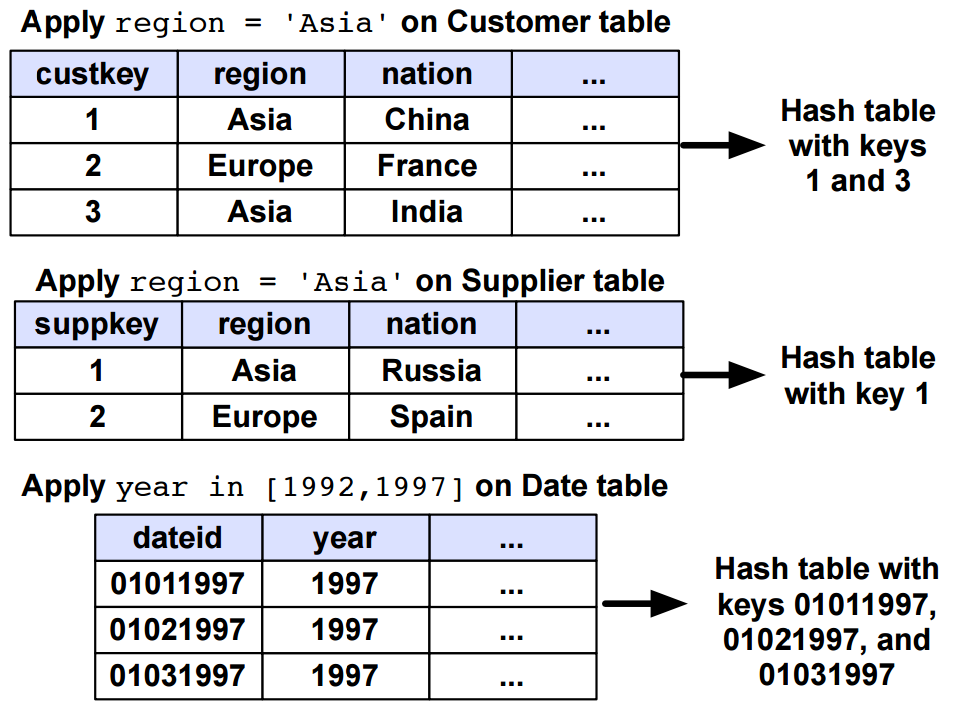
\includegraphics[width=\textwidth]{img/invisible-join-1.png}
    \caption{The first phase of the invisible join. Predicates are evaluated on every dimension table, and put into a hash map.}
    \label{fig:invisible-join-1} 
  \end{subfigure}
  \begin{subfigure}{0.45\textwidth}
    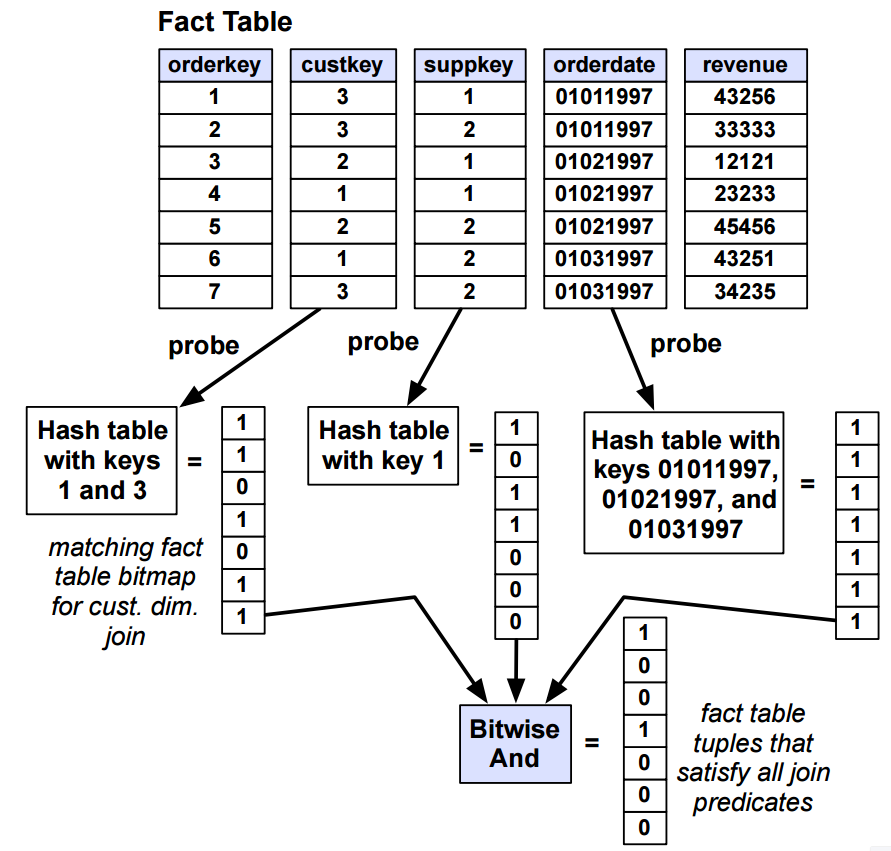
\includegraphics[width=\textwidth]{img/invisible-join-2.png}
    \caption{The second phase of the invisible join. Bitmaps are created per dimension table predicate, and bitwise \texttt{AND} is applied.}
    \label{fig:invisible-join-2} 
  \end{subfigure}
  \begin{subfigure}{0.45\textwidth}
    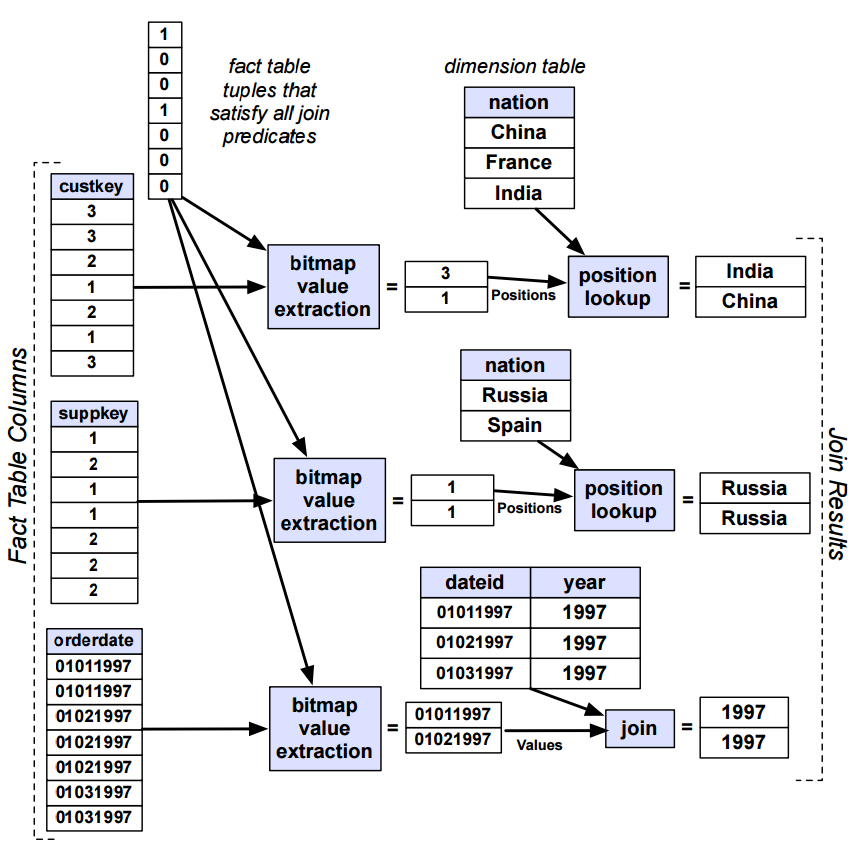
\includegraphics[width=\textwidth]{img/invisible-join-3.png}
    \caption{The third phase of the invisible join. The bitmap calculated in the previous step is uned to extract values from the fact table.}
    \label{fig:invisible-join-3} 
  \end{subfigure}
  \caption{The invisible join. Courtesy of \cite{Abadi2008-dd}.}
  \label{fig:invisible-join} 
\end{figure}
We chose to focus on a single algorithm for joining. We have no evidence that this algorithm is "the best", but it exemplifies how a join can be performed in a column store. In addition, it use some temporary bitmaps that can be cached. Introduced by Abadi \ea~in \term{invisible join} \cite{Abadi2008-dd}. Here, the set of tuples in the larger relation is reduced using selection predicates in one or many relation tables. For each predicate, a bitmap is produced. This is ANDed/ORed at the end of the query. Projected values are not fetched until the end. The whole join is depicted in Figure~\ref{fig:invisible-join}.

In this algorithm, bitmap filters based on foreign tables are created, which are similar to the join indexes discussed in section \ref{sec:Join Indexes}. We believe the intermediate result in this algorithm can be cached, as explained in Section \ref{sec:Caching and Dynamic Index Generation}.

\subsection{Bloom Filter Based Joins}
\label{sub:Bloom Filter Based Joins}
Although not directly compression, another way of reducing a bitmaps footprint and increasing query performance, is through the use of bloom filters \cite{Bloom1970-nr}. A bloom filter may return false positives, but never false negatives.The bloom filters can be used in common database operations, for instance joins \cite{x} \todo{Consider moving this somewhere else}. Several database systems report to use bloom filter based joins. Bloom filters, invented by Bloom in 1970, is a probabilistic structure and will only return false positives, not false negatives \cite{Bloom1970-nr}. This includes \oracle~\cite{Lahiri2015-mz}, \ibm~\cite{Raman2013-em}. Barber \ea~explain how bloom filters can be applied to eliminate non-matching join outers before they enter the join.

Since the inner table might be splitted, there is a large chance the key is not present in the relation when probed. Here, bloom filters can be used to determine if the matching key is not in the working space \cite{Bratbergsengen2015}. The use of bloom filters is encouraged if the inner relation is partitioned, to avoid going into the hash structure.

\subsection{Parallel Joining}
\label{sub:Parallel Joining}
Joining becomes a challenge when done in parallel.

In \ibm, each thread performs a local grouping on a local hash tables and creates a linked list of overflow buckets \cite{Raman2013-em}. When they are full, they get published globally. Second phase, each thread reserves a partition to merge, and it merges all local hash tables to a global one.

The hash tables can be built in parallel \cite{Barber2014-ey}. Hyperthreading will speed up the probe phase \todo{Because the memory gap is hidden?}.

Several join algorithms discussed in Section X partitions the input in order to improve cache locality. This decision might as well be a parallelization decision \cite{Neumann1011-uq}.

\section{Grouping and Aggregation}
\label{sec:Grouping and Aggregation}
Conceptually, grouping and aggregation is relatively straight forward: The record set is scanned and divided into groups based on one or more attributes, and for each group an accumulator is held \cite{Bratbergsengen2015-ed}. Accumulators can be of various types, which includes \term{count}, \term{min}, \term{max}, \term{average}, and \term{sum}. Some aggregates require just a single memory cell, like \term{count} and \term{sum}, others are more involved and require more memory to calculate, like \term{median} and \term{average}. Aggregated results are stored in a suitable structure, like a hash table or linear array. 

Multiple optimizations can be done to improve grouping and aggregation performance. First, the operations can be applied at the same time as for the scan \cite{Lemke2010-is}. This is done in \blink, where the core idea is a generalized scan that filters, groups, and aggregates on a single scan over the data \cite{Raman2008-gi}.

Dictionary encoding can simplify grouping and aggregation, since dictionary entries can be used directly for storing the aggregated results \cite{Boncz2005-wj, Lemke2010-is}. This is done in \monetx~and \blink. \blink~uses dictionary codes directly as group codes. Doing such results in a perfect hash \cite{Raman2008-gi}. Also, some aggregates, like minimum and maximum value in a column, can be evaluated scanning only  dictionary entries \cite{Lemke2010-is}.

\ffigure{img/vector-group-by}{The \term{Vector Group By} technique used in \oracle. Courtesy of \cite{Oracle2015-fs}.}{fig:vector-group-by}
On composite \texttt{GROUP BY} operations, a multidimensional structure may be used. \oracle~uses a technique which they call \term{Vector Group By}, which is a compact multipdimensional array for storing aggregate results. The operation is depicted in Figure~\ref{fig:vector-group-by}. \blink~calculates a minimal perfect hash in this case \cite{Raman2008-gi}.

\ffigure{img/parallel-group-by}{Courtesy of \cite{Raman2013-em}.}{fig:parallel-group-by}
If the columns are partitioned horizontally, grouping and aggregation must be performed in two phases: A scan phase per partition followed by a global merge phase \cite{Lemke2010-is}. In a distributed system, the grouping is even more involved. For \ibm, local grouping is performed per node in parallel \cite{Raman2013-em}\todo{elaborate}. In \exasol~and \oracle, an attribute in a table might specifiy table partitioning \cite{Exasol2014-xh, Lahiri2015-mz}. If a query is grouped by the same attribute, the work is already done.

As mentioned in Section \ref{sub:Queries}, in \bd~workloads, the groups will be predefined in the panel. However, new aggregation results must be populated when filters are applied.

\subsection{Parallel Grouping and Aggregation}
\label{sub:Parallel Grouping and Aggregation}
Vendors say their grouping operations scale linearly with the number of threads until the CPU is saturated \cite{Farber2012-vh}

In \ibm~, each thread performs a local grouping on a local hash tables and creates a linked list of overflow buckets \cite{Raman2013-em}. When they are full, they get published globally. Second phase, each thread reserves a partition to merge, and it merges all local hash tables to a global one.

\section{Query Optimization}
\label{sec:Query Optimization}
Our study of query optimization will be brief, but we have found some sources relevant for OLAP workloads. Most of the database systems found in literature use some kind of query optimization. 

In general, query optimizers must seek to reduce the search space \cite{Boncz2002-yj, Stonebraker2005-qz}. \blink~makes query optimization much easier, since the only operation for evaluating predicates in a query is a scan operation \cite{Barber2012-xt}. In addition, joins and grouping is done in prespecified order. The core idea of this system is a generalized scan which performs scan, selection, groping, and aggregation \cite{Raman2008-gi}. 

If compression is applied to the database, it is important that the optimizer is aware \cite{Westmann200-mz}. The query optimizer must be aware that columns might be compressed, and that these compressed columns can be worked on directly without decompression \cite{Stonebraker2005-qz}

In addition, it is important to filter data as early as possible in the plan \cite{Lamb2012-kg}, and in join operation  most selective columns should be processed first \cite{Holloway2008-rr}. In a parallel settiong, the query optimizer should minimize the need for coordination \cite{Exasol2014-xh}.

Long in-lists can be turned into a precomputed hash table \cite{Raman2013-em}.

We conclude our discussion on query optimization that query execution must utilize available optimizations allowed by the design. Metadata indexes (Section ?) can be used to skip blocks. Dictionaries can be checked, and partitions can be skipped entirely if the key is not present in the dictionary (Section ?). \texttt{LIKE} predicates can be turned into \texttt{IN} predicates based on the entries in the dictionary.

%\section{Query structures}
%\label{sec:Query structures}
%\missingfigure{Selection vector illustration from \cite{Boncz2005-wj}}
%If the queries work on vectors at a time (vectorized execution, section X), the auxiliary structure in \monetx~is a selection vector \cite{Boncz2005-wj}.

\section{Other Considerations}
\label{sec:Other Considerations}
We find one of the most important technique for good query performance to operate directly on compressed data, which we have studied in Section \ref{sub:Working Directly on Compressed Data}. As we have seen, this is especially important when using dictionary compression, such that most predicates can be performed by simple integer operations \cite{Abadi2008-dd}. If the data is bitpacked, queries can be processed in a SIMD-like fashion, a technique we study in more detail in Section \ref{sec:SIMD}. Systems querying direcly on compressed data include \cstore~\cite{Stonebraker-qz}, \ibm~\cite{Raman2013-em}, \mssql~\cite{Larson2013-mc}, \blink~\cite{Johnson2008-cp}, \sapnw~\cite{Lemke2010-is}. All of these systems claim one of their main benefits in terms of performance is their ability to work directly on the compressed data.


We see that some systems make a distinction between measure and dimension attributes \cite{Kamkolkar2015-iq, Johnson2008-cp}. A dimension attribute is typically answers questions like "where", "what", and "when", whereas a measure attribute nomally answers in terms of "how much" \cite{noauthor_undated-es}. Although we have no specific evidence of what this classification can do to aid query processing, we believe it can help determine data placement and which results that are cached. For dimensions, join indexes and filtered results are obvious candidates for caching. In a banked layout, used in \blink, or in column projections, used in \cstore, dimension attributes should be put together in the same bank or projection to aid predicate evaluation. Measure attributes on the other hand are candidates for caching of query results

\subsection{Query Restrictions}
\label{sub:Query Restrictions}
Most DBMSes support normal SQL operations. However, to simplify some of the queries, one may put restrictions to the SQL. Earlier versions of \mssql~did not support outer joins and group-by on scalar attributes \cite{Larson2013-mc}. This was justified as none of this was common for "datawarehouse scenarios".

Other work has suggested that standard SQL can be cumbersome and expensive \cite{Plattner2014-fr}, and want to investigate new ways of calculating and maintaining a database. \qlikview~is not in the \term{query-based paradigm}, and claims this is beneficial due to ... \todo{insert reasons here}

\bd~applications do not need to support all SQL operations which a DBMS normally does. For instance, joins can be limited to equi-joins over foreign keys, and aggregations may be limited to groups of one or more dimensions in the schema.

\section{Predicate Evaluation}
\label{sec:Predicate Evaluation}
We see various techniques that improves the predicate evaluation.

It is common to use bitmaps in predicate evaluation \cite{Raman2008-gi, Raman2013-em}. In \blink, bitmaps are calculated and operations are performed directly on the bitmaps.

Predicates are also evaluated in a Single Input Multipe Data (SIMD) fashion, which is a technique described by Johnson \ea~\cite{Johnson2008-cp}. Extensive use of processor SIMD instructions is explained by Willhalm \ea~\cite{Willhalm2009-hu, Willhalm2013-ri}. Evaluating predicates in a SIMD like fashion is done in \blink~\cite{Raman2008-gi}.  This system reports a performance increase when three or more predicates are evaluated at the same time.

\subsection{Predicate Evaluation in Parallel}
\label{sub:Predicate Evaluation in Parallel}
\blink~runs all predicates in parallel, with no pipelining \cite{Raman2008-gi}.

\section{Chapter Conclusion}
\label{sec:Chapter Conclusion}
We conclude this chapter that join should be executed using a \term{nested loop} algorithm. This type of algorithm is suited for joins where tables fit in memory, which we assume. We also recommend adding Bloom filters to the structures to limit the number of keys entering the join. We recommend using a technique similar to Abadi \ea's \algmet{Invisible Join} for joining.

We also encourage investigating the benefits of caching temporary structures used in both cache and aggregation. In the case of \algmet{Invisible Join}, the predicate bitmaps can be cached.

Queries must also work directly on compressed data, as concluded in Chapter \ref{chp:Compression}.
